\documentclass{beamer}

\usepackage{amsmath}
\usepackage{amsfonts}
\usepackage{amssymb}
\usepackage{listings}
\usepackage{graphicx}
\usepackage{tikz}
\usepackage{url}
\usepackage{array}
\usepackage{qrcode}

\graphicspath{{../}}

% KCPC theme
\usetheme{default}
\useinnertheme{rectangles}
\useoutertheme{default}

\beamerdefaultoverlayspecification{<1->}

\setbeamertemplate{navigation symbols}{}

% Colours
\definecolor{kcpc-bg}{RGB}{250,250,250}
\definecolor{kcpc-text}{RGB}{20,20,20}
\definecolor{kcpc-muted}{RGB}{90,90,90}
\definecolor{kcpc-red}{RGB}{176,0,0}

\setbeamercolor{background canvas}{bg=kcpc-bg}
\setbeamercolor{normal text}{fg=kcpc-text}
\setbeamercolor{frametitle}{fg=kcpc-text,bg=kcpc-bg}
\setbeamercolor{title}{fg=kcpc-text}
\setbeamercolor{subtitle}{fg=kcpc-muted}
\setbeamercolor{structure}{fg=kcpc-red}

\setbeamerfont{title}{series=\bfseries,size=\Large}
\setbeamerfont{frametitle}{series=\bfseries,size=\large}

\setlength{\parskip}{0.4em}

\setbeamertemplate{itemize item}{$\rightarrow$}
\setbeamertemplate{itemize subitem}{$\rightarrow$}

\setbeamertemplate{headline}{
    \vspace{0.2cm}
    \hspace{0.2cm}
    \textcolor{kcpc-muted}{\small Problems and Materials}
    \hfill
}

\setbeamertemplate{footline}{
    \hspace{0.2cm}
    \textcolor{kcpc-muted}{\small KCPC}
    \hfill
    \vspace{0.3cm}
}

\setbeamertemplate{background}{
    \begin{tikzpicture}[remember picture,overlay]
        \node[
            opacity=0.035,
            at=(current page.center)
        ] {
            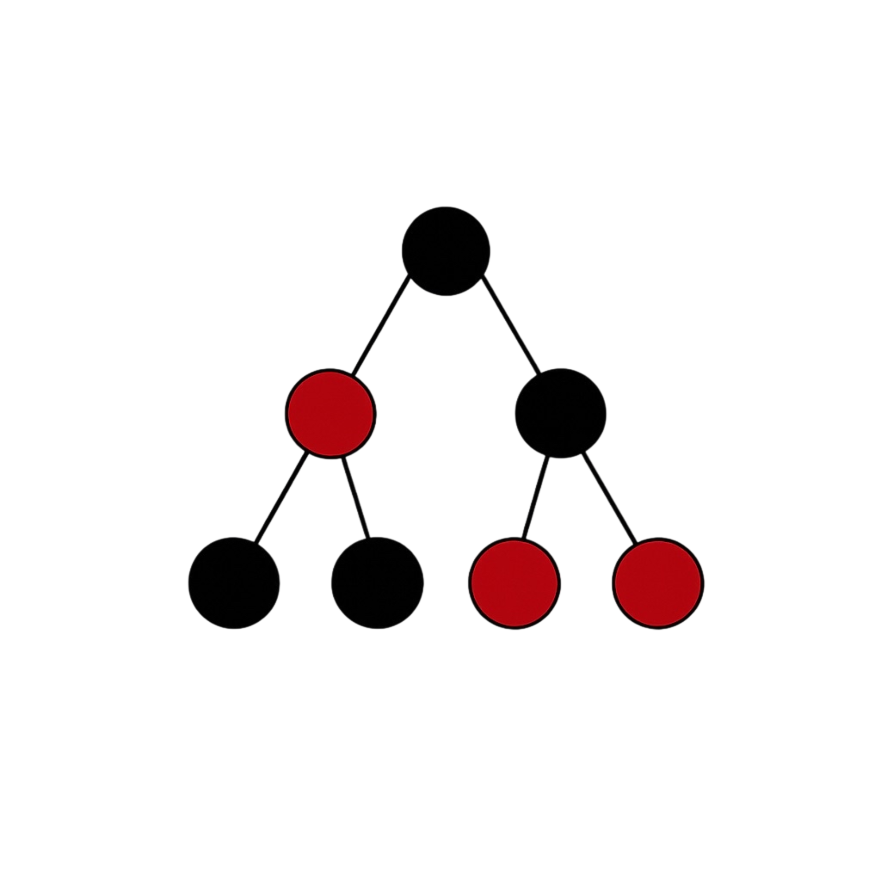
\includegraphics[width=0.55\paperwidth]{kcpc-logo.png}
        };
    \end{tikzpicture}
}

\title{UKIEPC 2026}
\subtitle{Hacking Session 1}
\author{KCPC}
\date{21 October 2026}

\newcommand{\problemframe}[5]{%
    \begin{frame}{Problem #1: #2}
        \textbf{Problem:} #3\par
        \vspace{0.5em}
        \textbf{Solution:}
        \begin{itemize}
            \setlength{\itemsep}{0.25em}
            #4
        \end{itemize}
        \vfill
        {\small\textcolor{kcpc-muted}{Time complexity: #5}\par}
    \end{frame}
}

\begin{document}

\begin{frame}
    \titlepage
\end{frame}

\begin{frame}[fragile]{Problems and Materials}
    \begin{columns}[c]
        \begin{column}{0.55\textwidth}
            The UKIEPC 2026 problem sheet for KCPC Year 2 Hacking Session 1.
            \par\vspace{0.8em}
            Scan the QR code to open the official problem booklet.
            \par\vspace{0.8em}
            {\scriptsize\url{https://github.com/orthant-kcpc/kcpc-workshops/blob/main/KCPC\%20Year\%202\%20Workshops/Hacking\%20Session\%201/Hacking\%20Session\%201\%20Problems.pdf}}
        \end{column}
        \begin{column}{0.4\textwidth}
            \centering
            \qrcode*[height=4.3cm]{https://github.com/orthant-kcpc/kcpc-workshops/blob/main/KCPC%20Year%202%20Workshops/Hacking%20Session%201/Hacking%20Session%201%20Problems.pdf}
        \end{column}
    \end{columns}
\end{frame}

\problemframe{E}{Elderberry Wine}
    {Find the total ingredients to order so that the stock can be brewed in the required $12:12:40$ ratio.}
    {\item<1-> Every initial ingredient is eventually used; the limiting ingredient determines $M=\max(a/12,b/12,c/40)$.
     \item<1-> The final stock must be $(12M,12M,40M)$, so order each positive deficit.
     \item<1-> Use extended precision, or defer division, for inputs up to $10^{16}$.}
    {$O(1)$}

\problemframe{A}{Austere Sign}
    {Rewrite the sign using at most $k$ distinct letters, changing as few letters as possible without changing any word lengths.}
    {\item<1-> Count each letter's frequency across all words in linear time.
     \item<1-> Keep the $k$ most frequent letters to minimise replacements.
     \item<1-> Replace every other letter with a kept letter.}
    {$O(N)$}

\problemframe{I}{Inverse Sum}
    {Find distinct positive integers $a,b$ with minimum sum such that $1/n=1/a+1/b$.}
    {\item<1-> Rearranging gives $(a-n)(b-n)=n^2$.
     \item<1-> Set $x=a-n$ and $y=b-n$; minimise $x+y$ over distinct factor pairs of $n^2$.
     \item<1-> Factor $n$ in $O(\sqrt n)$ and choose the largest divisor $x<n$ of $n^2$, with $y=n^2/x$.}
    {$O(\sqrt n+d(n^2))$}

\problemframe{C}{Cryptlet}
    {Assign distinct digits to the five letters so that the given equal-length addition $X+Y=Z$ is valid.}
    {\item<1-> Only $10!/5!=30{,}240$ distinct digit assignments need testing.
     \item<1-> Precompute each letter's positional-weight sum modulo large primes in $O(|X|)$.
     \item<1-> Check each assignment with constant-time modular combinations and verify candidates with two additional primes.}
    {$O(|X| + 30{,}240)$}

\problemframe{K}{Kilt Quilt}
    {Find a shortest sequence of full-row and full-column brush strokes that paints a given canvas.}
    {\item<1-> Every cell must be covered; assume without loss of generality that all rows are painted.
     \item<1-> Any untouched column reveals the required colour of every row stroke.
     \item<1-> A mismatch forces row/column stroke precedence; topologically sort these constraints and report impossible if they cycle.}
    {$O(N^3)$}

\problemframe{F}{Footnotes}
    {Move exactly two-thirds of the letters in a nested-bracket string into two equally sized footnotes.}
    {\item<1-> Let $L$ be the total number of letters; if $3\nmid L$, the answer is impossible.
     \item<1-> Parse the brackets into a syntax tree and count letters in every subtree in $O(|s|)$.
     \item<1-> Check for two disjoint $L/3$ subtrees, or an $L/3$ subtree nested inside a $2L/3$ subtree.}
    {$O(|s|)$}

\problemframe{B}{Bust Blasting}
    {Find the volume of the 3D shape that remains after intersecting the statue's front, side, and top projections.}
    {\item<1-> Coordinate-compress each axis, leaving at most 200 intervals per axis.
     \item<1-> Rasterise each 2D projection as a $200\times200$ mask using the even/odd fill rule.
     \item<1-> Sum $\Delta x\,\Delta y\,\Delta z$ for each cuboid active in all three masks.}
    {$O(N^3)$, optimisable to $O(N^2)$}

\problemframe{G}{Gloucester Somersault}
    {Count the full revolutions needed for a rolling polygonal cheese to cross the finish line while touching the ground.}
    {\item<1-> Interior vertices never touch the ground, so the rolling distance is determined by the convex hull.
     \item<1-> One full revolution advances the cheese by the convex-hull perimeter $P$.
     \item<1-> From the initial rightmost ground contact $x_0$, round up $(m-x_0)/P$; the official notes warn strict-boundary cases were absent from contest tests.}
    {$O(N\log N)$}

\problemframe{L}{Lawn Stripes}
    {Route a roller over a square lawn so every cell ends with its requested cardinal direction.}
    {\item<1-> Give each cell one outgoing edge in its required direction; the lawn becomes a functional graph.
     \item<1-> Following edges from the start reaches a cycle or boundary sink; reverse edges to form trees rooted there.
     \item<1-> DFS an Euler-style tour of the trees to cover all cells within the $10n^2$ move limit.}
    {$O(N^2)$}

\problemframe{H}{Hoptimisation}
    {Arrange up to 16 cell names along a line to minimise the total distance of a given sequence of hops.}
    {\item<1-> This is minimum linear arrangement; $k\le16$ makes an exponential subset DP feasible.
     \item<1-> Rewrite total travel as the sum, over line boundaries, of transitions crossing each cut.
     \item<1-> Use $\mathrm{dp}[S]=\min_{v\in S}(\mathrm{dp}[S\setminus\{v\}]+\mathrm{cutCost}[S])$ and retain choices to recover the order.}
    {$O(N+2^k k)$}

\problemframe{M}{Mid Clocking}
    {Place tasks in processor slots to minimise the finishing time when adjacent processors run more slowly.}
    {\item<1-> Binary-search a candidate makespan $T$.
     \item<1-> A task with $t/0.6>T$ needs zero neighbours; if $t/0.3>T$, it can have at most one.
     \item<1-> Check whether these task classes fit the optimal patterns of isolated slots, adjacent pairs, and dense $30\%$ blocks.}
    {$O(N\log N+\log(\text{range}/\varepsilon)\log N)$}

\problemframe{J}{Jammer Jam}
    {Assign swimmers to lanes to maximise their average speed when everyone in a lane ends up matching its slowest swimmer.}
    {\item<1-> Sort by speed; an optimal lane is a contiguous interval $[i,j]$ with total speed $(j-i+1)a_i$.
     \item<1-> Dynamic programming chooses interval boundaries for each lane, but the direct transitions are too slow.
     \item<1-> Convexity/quadrangle structure enables divide-and-conquer or convex optimisation; Lagrange relaxation can reduce dependence on the lane count.}
    {$O(N\log N)$ or $O(N\log(\text{range}))$}

\problemframe{D}{Dire Strait}
    {Find the shortest path between two vertices inside a simple polygon when a triangulation is given.}
    {\item<1-> The dual graph of the triangulation is a tree, so the endpoints have a unique triangle strip (the sleeve).
     \item<1-> Treat the strip's interior edges as portals and tighten a visibility funnel through them.
     \item<1-> When the funnel collapses, take the blocking corner and continue through the remaining portals.}
    {$O(N)$}

\end{document}
